% !TeX spellcheck = <none>
\documentclass{report}
\usepackage{graphicx}
\usepackage[portuguese]{babel}
\usepackage[utf8]{inputenc}
\usepackage{hyperref}
\usepackage{indentfirst}
%\usepackage[latin1]{inputenc}
%\usepackage{url}
\usepackage{color}
\usepackage{enumerate}
\usepackage{alltt}
\usepackage{fancyvrb}
\usepackage{listings}
\usepackage{amsmath}
\newcommand{\keyword}[1]{\textsf{#1}}

\DefineVerbatimEnvironment{code}{Verbatim}{fontsize=\footnotesize}
%LISTING - GENERAL
\lstset{
	basicstyle=\small,
	numbers=left,
	numberstyle=\tiny,
	numbersep=5pt,
	breaklines=true,
    frame=tB,
	mathescape=true,
	escapeinside={(*@}{@*)}
	}


\title{Processamento de Linguagens e Compiladores\\ (3º ano de LCC)\\ \textbf{Desenvolvimento de Linguagem de Programação}\\ TP3\\ Grupo 14}
\author{Artur Queiroz\\ A77136 \and  Rafael Fernandes\\ A78242 \and Rafaela Pinho\\ A77293 }
\date{\today}

\begin{document}
	
\maketitle
	

\begin{abstract}
	Neste relatório apresentamos a linguagem que criamos, o Galo, e o complidor que gera o código para a Máquina Virtual VM.
\end{abstract}

\tableofcontents

\chapter{Introdução} \label{intro}
\indent
Neste relatório apresentamos o último trabalho da unidade curricular "Processamento de Linguagens e Compliadores". Este consiste em desenvolver um processador de linguagens usando o método da tradução dirigida pela sintaxe. Também devemos desenvolver um compilador que gera o código para uma máquina de stack virtual. Utilizaremos a ferramenta Yacc para gerar compiladores baseados em gramáticas tradutoras.\\
\indent
Como todos os outros trabalhos, este também tem como objetivo aumentar a experência no uso do ambiente Linux, da linguagem C e  ferramentas de apoio à programção.\\
\indent
Este relatório está dividido em 4 partes. No primeiro capítulo encontramos a parte introdutório a este trabalho, onde explicamos no que consiste. No capítulo 2 (dois) apresentamos os requisitos e a linguagem que criamos. No terceiro mostramos as decisões e alguns teste efectuados. No último temos a conclusão e os objetivos do trabalho futuro.
 
\chapter{Galo e Compilador} \label{fi}
\section{Descrição informal do problema}
\indent
Neste trabalho foi pedido para criarmos uma linguagem de programação imperativa e desenvolver um compilador para a linguagem criada.\\
\indent
Na linguagem as declarações de variáveis devem ser colocadas no início do programa, não pode haver re-declarações e não se pode usar variáveis sem estar declaradas primeiro. Caso não seja atribuido um valor à variável depois da declaração, esta ficará com o valor zero se for um inteiro, se for um float ficará 0.0 e se for string ficará $"$".\\
\indent  	
O complilador deve gerar o código assembly para a Máquina Virtual VM.

\section{Especificação dos requisitos}
\indent
Para este trabalho a linguagem que criamos tem de conter os seguintes requisitos:
\begin{enumerate}
	\item Declarar e manusear variáveis atómicas do tipo inteiro e estruturas do tipo array de inteiros.
	\item Ler do standard input e escrever no standard output.
	\item Fazer instruções básicas como a atribuição de expressões a variáveis.
	\item Definir e invocar subprogramas sem parâmetros mas que possam retornar um resultado atómico.
	\item Efetuar instruções para controlo do fluxo de execução — condicional e cíclica — que possam ser aninhadas.
\end{enumerate}
\indent
Também deverá conter um conjunto de testes (escritos na nossa linguagem) que tem de ter no mínino os 6 exemplos seguintes:
\begin{enumerate}[i)]
	\item Ler 4 números e dizer se podem ser os lados de um quadrado.
	\item Ler um inteiro N, depois ler N números e escrever o menor deles.
	\item Ler N (constante do programa) números e calcular e imprimir o seu produtório.
	\item Contar e imprimir os números ímpares de uma sequência de números naturais.
	\item Ler e armazenar os elementos de um vetor de comprimento N; imprimir os valores por ordem decrescente após
	fazer a ordenação do array por trocas diretas.
	\item Ler e armazenar N números num array; imprimir os valores por ordem inversa
\end{enumerate} 
\section{Expressões regulares} 
As expressões regulares usadas foram:

\begin{enumerate}
	\item \#.*\$  
	\item $\backslash$"[\^\"]* $\backslash$"
	\item $[$ $]$+e$[$ $]$+
	\item $[$ $]$+ou$[$ $]$+
	\item $[$ $]$+sin$[$ $]$+
	\item $[$ $]$+cos$[$ $]$+
	\item ==
	\item $\backslash$$<=$
	\item $\backslash$$>=$
	\item !=
	\item $[$=;\{\}(),$<>$!$\backslash$+$\backslash$-$\backslash$*$\backslash$/\%$\backslash$[$\backslash$]]
	\item se$|$SE
	\item senao$|$SENAO 
	\item enq$|$ENQ
	\item return
	\item $[$0-9]+$\backslash$.[0-9]+ 
	\item int$|$string$|$float 
	\item -?$[$0-9]+
	\item $[$a-zA-Z][a-zA-Z0-9]*
	\item $[$$\backslash$t$\backslash$n] 
	
\end{enumerate}

\section{A nossa linguagem}
\subsection{Galo}
\indent
Como já referido em cima, foi-nos pedidos para criar uma linguagem de programação. Decidimos chamar de Galo por ser um símbolo típico de Potugal, e atribuimos *.gal para a extensão. Para a construção da nossa linguagem fomos inspirados pela pseudo linguagem usada nas aulas pelos professores.
\indent
Para a definir utilizamos uma gramática independente do contexto, em que tomamos certas decisões que serão especificadas mais à frente.\\
\indent
O Galo reconhece os segintes tipos: números inteiros (int), números décimais  (float) e sequência de caractéres (string). A linguagem usa os habituais símbolos de comparação, como $<=$, $>=$, $<$, $>$, $==$ e $!=$. Utiliza o "e" e o "ou" como símbolos de operadores lógicos.\\
\indent
Como a nossa linguagem é muito parecida ao C, para fazer o "ite" utilizamos o "se" e o "senao" (tanto minúsculo como maiúsculo) para o "while" usamos o "enq" ou "ENQ".\\
\indent
Existe as funções "ler?()" e "escrever?()" que são, respetivamente, a função de leitura no teclado e de escrita no ecrã. (? = i ou s ou f, i-inteiro, s-string, f- float) \\

\indent
A nossa linguagem está definida pela seguinte GIC:

\begin{code}
	
	1 ProgG: ProgG Se
	2      | ProgG Enq
	3      | ProgG Atrib ';'
	4      | ProgG VAR '=' Expr ';'
	5      | ProgG VAR '[' Expr ']' '=' Expr ';'
	6      | ProgG CriaFun
	7      | ProgG Funcao ';'
	8      | ProgG ';'
	9      | ProgG COM
	10     | %empty
	
	11 ProgF: ProgF Se
	12      | ProgF Enq
	13      | ProgF Atrib ';'
	14      | ProgF VAR '=' Expr ';'
	15      | ProgF VAR '[' Expr ']' '=' Expr ';'
	16      | ProgF Funcao ';'
	17      | ProgF ';'
	18      | ProgF COM
	19      | ProgF RETURN Expr ';'
	20      | %empty
	
	21 Prog: Prog Se
	22     | Prog Enq
	23     | Prog Atrib ';'
	24     | Prog VAR '=' Expr ';'
	25     | Prog VAR '[' Expr ']' '=' Expr ';'
	26     | Prog Funcao ';'
	27     | Prog ';'
	28     | Prog COM
	29     | %empty
	
	30 Funcao: VAR Lexpr
	
	31 CriaFun: TIPO VAR '('
	32        | Ltipo '{' ProgF '}'
	
	33 Atrib: TIPO VAR
	34      | TIPO VAR '[' Expr ']'
	35      | Igual
	
	36 Igual: TIPO VAR '='
	37      | TIPO VAR '[' Expr ']' '='
	38      | Igual Expr
	
	39 Lexpr: '(' ')'
	40      | '(' Eexpr ')'
	
	41 Eexpr: Expr
	42      | Eexpr ',' Expr
	
	43 Ltipo: ')'
	44      | Etipo ')'
	
	45 Etipo: TIPO VAR
	46      | Etipo ',' TIPO VAR
	
	47 Se: SE Cond
	48   | Se '{' Prog '}' SENAO
	49   | Se '{' Prog '}'
	
	50 Enq: ENQ
	51    | Enq Cond
	52    | Enq '{' Prog '}'
	
	53 Cond: NUM
	54     | '(' Expr EQ Expr ')'
	55     | '(' Expr NEQ Expr ')'
	56     | '(' Expr '<' Expr ')'
	57     | '(' Expr '>' Expr ')'
	58     | '(' Expr LEQ Expr ')'
	59     | '(' Expr GEQ Expr ')'
	60     | '(' Cond E Cond ')'
	61     | '(' Cond OU Cond ')'
	62     | '!' Cond
	
	63 Sexpr: VAR
	64      | NUM
	65      | FLOAT
	66      | VAR '[' Expr ']'
	67      | Funcao
	68      | STR
	
	69 Expr: '(' Expr '+' Expr ')'
	70     | '(' Expr '-' Expr ')'
	71     | '(' Expr '*' Expr ')'
	72     | '(' Expr '/' Expr ')'
	73     | '(' Expr '%' Expr ')'
	74     | COS Expr
	75     | SIN Expr
	76     | '(' Expr ')'
	77     | Sexpr
	
\end{code}

\chapter{Codificação e Testes}
\section{Problemas de implementação, Decisões e Alternativas}
\subsection{Problemas de implementação}
\indent
Como em todos os trabalhos tivemos alguns contratempos, dos quais muitos foram superados.\\
\indent
Quando estavamos a passar a nossa linguagem para uma gramática tradutora tivemos alguns problemas com o código assembly da máquina virtual, mas nada que não se resolvesse com um bocadinho de paciência e trabalho de grupo.\\
\indent
Tivemos problemas com a implementaçáo de vetores, pois nao conseguimos compreender a forma de utilização correcta do comando load, não conseguindo completar o exemplo 5 e 6.  Após uma oportunidade por parte dos professores e um esclarecimento conseguimos resolver os problemas ficando o exemplo 5 e 6 a funcionar.
   
\subsection{Decisões}
\begin{enumerate}[1)]
	\item O "e" ($\&\&$) está definida pela multuplicação e o "ou" ($||$) pela adição.
 
	 \begin{table}[h]
		\begin{center}
	 	\caption{Tabela do E}
	 	\begin{tabular}{r|lr}
	 	 *(E)& 0 & 1\\ % Note a separação de col. e a quebra de linhas
	 	\hline          % para uma linha horizontal
	 	0 & 0 & 0 \\
	 	1 & 0 & 1\\
 	
		\end{tabular}
		\caption{Tabela do OU}
		\begin{tabular}{r|lr}
		+(OU)& 0 & 1\\ % Note a separação de col. e a quebra de linhas
		\hline          % para uma linha horizontal
		0 & 0 & 1 \\
		1 & 1 & 2\\
		\end{tabular}
		\end{center}
	\end{table}

	\item Não se pode declarar mais do que uma variável numa linha, ou seja todas as declarações são individuais.\\
	 Exemplo: \\int a = 2 , c = 0;\\ terá de ser:\\
	 int a = 2;\\
	 int c = 0;\\
	 \item Não se pode fazer "return" dentro dos Se's e dos Enq's.\\ 
	 \item Nas expressões numéricas, as operações binárias têm de estar sempre dentro de parênteses.\\
	 Exemplo:\\
	 int a = (1+(2*3));
	 \item Todo o código dentro de se's, enq's e funções começa em '$\{$' e acaba em  '$\}$'.
	 
	
\end{enumerate}

\section{Testes realizados e Resultados}
\subsection{Exemplos escritos na nossa linguagem}

\begin{enumerate}
	\item Ler 4 números e dizer se podem ser os lados de um quadrado.\\
	
	\begin{code}
		int a = leri();
		int b = leri();
		int c = leri();
		int d = leri();
	
		se ((a==b) e ((b==c) e (c==d))) {
			escrevers("É um quadrado\n");
		}
		senao {
			escrevers("Não é um quadrado\n");
		}
	\end{code}	
	
	\item Ler um inteiro N, depois ler N números e escrever o menor deles.\\
	
	\begin{code}
		escrevers("Escreva o número de elementos do array:\n");
		int N = leri();
		
		int i = 0;
		int a = 0;
		int res = 0;
		
		se (N>0){
			res = leri();
			i = 1;
			enq (i < N){
				a = leri();
				
				se (res > a){
					res = a;
				}
				
				i = (i+1);
			}
			
			
			escrevers("O menor número foi o ");
			escreveri(res);
			escrevers("\n");
			
		}
		senao{
			escrevers("Não leu nenhum número\n");
		}
	\end{code}
	
	\item Ler N (constante do programa) números e calcular e imprimir o seu produtório.\\
	
	\begin{code}
		escrevers("Vão se ler 5 números\n");
		
		int N = 5;
		int i = 0;
		int r = 1;
		
		enq(i < N){
			
			r = (r * leri());
			
			i = (i + 1);
		}
				
		escrevers("O produtório desta sequencia de 5 números é ");
		escreveri(r);
		escrevers("\n");
	\end{code}

	\item Contar e imprimir os números ímpares de uma sequência de números naturais.\\
	
	\begin{code}
		escrevers("Digitar uma sequência de números, termina quando for zero\n");
		
		int cont = 0;
		int i = leri();
		
		enq(i != 0){
			se ((i % 2) == 1){
				cont = (cont + 1);
				escreveri(i);
				escrevers(" \n");
			}
			i = leri();
		}
	
		escrevers("Foram lidos ");
		escreveri(cont);
		escrevers(" ímpares \n");
	\end{code}
 
  	\item Ler e armazenar os elementos de um vetor de comprimento N; imprimir os valores por ordem decrescente após
	fazer a ordenação do array por trocas diretas.\\
	
	\begin{code}
	
	
	int i = 0;
	int v[20];
	
	escrevers("Introduza um numero natural menor que 20\n");
	int N = leri();
	
	
	se((0>=N) ou (N>20)){
		escrevers("OOps, parece que tivemos uns problemas, 0<N<=20.\n");
	}senao{
		enq(i<N){
			v[i] = leri();
			i = (i+1);
		}
		
		int changed = 1;
		int k;
		enq (changed == 1) {
			changed = 0;
			i = 0;
			enq (i<(N - 1)){
				se(v[i]<v[(i+1)]){
					k = v[i];
					v[i] = v[(i+1)];
					v[(i+1)] = k;
					changed = 1;
				}
				i = (i+1);
			}
		}
		
		i = 0;
		enq(i<N){
			escreveri(v[i]);
			escrevers(" \n");
			i = (i+1);
		}
	}
	
	
	\end{code}	
	
	\item Ler e armazenar N números num array; imprimir os valores por ordem inversa.\\
	
	\begin{code}
		int i = 0;
		int a = 0;
		int v[20];
		
		
		escrevers("Introduza um numero inteiro positivo e inferior a 20.\n");
		int N = leri();
		
		se ((0>=N) ou (N>20)){
			escrevers("OOps alguem esta a tentar ser rebelde.\n");
		}senao{
			enq (i < N){
				v[i] = leri();
				i = (i + 1);
			}
			
			enq(i > 0){
				a = v[(i-1)];
				escreveri(a);
				escrevers(" \n");
				i = (i-1);
			}
		}
	\end{code}

\end{enumerate}

\subsection{Resultados}
\indent
Depois de executarmos os comados seguintes:\\
\noindent
\$ flex -o galo.c galo.l\\
\$ yacc -d -v galo.y\\
\$ gcc -o galo y.tab.c -lm\\
compilamos todos os nossos exemplos.\\
\indent
Obtivemos o seguinte resultado:
\begin{enumerate}
	\item Ler 4 números e dizer se podem ser os lados de um quadrado.
	\begin{code}
		
	start
	pushi 0
	read
	atoi
	storeg 0
	pushi 0
	read
	atoi
	storeg 1
	pushi 0
	read
	atoi
	storeg 2
	pushi 0
	read
	atoi
	storeg 3
	pushg 0
	pushg 1
	equal
	pushg 1
	pushg 2
	equal
	pushg 2
	pushg 3
	equal
	mul
	mul
	jz fimse0
	pushs "É um quadrado\n"
	writes
	jump fimse1
	fimse0:
	pushs "Não é um quadrado\n"
	writes
	fimse1:
	stop
	
	\end{code}
	\indent
	Após abrir o ficheiro na máquina virtual, se atribuirmos, por exemplo, o número 4 ao a, b, c, d o programa retorna \textbf{"É um quadrado"} (Figura A.1). Se atribuinos valores diferentes ao a, b, c, d o programa diz \textbf{"Não é um quadrado"} (Figura A.2).
	
	
	\item Ler um inteiro N, depois ler N números e escrever o menor deles.
	
	\begin{code}
		start
		pushs "Escreva o número de elementos do array:\n"
		writes
		pushi 0
		read
		atoi
		storeg 0
		pushi 0
		pushi 0
		storeg 1
		pushi 0
		pushi 0
		storeg 2
		pushi 0
		pushi 0
		storeg 3
		pushg 0
		pushi 0
		equal
		pushi 0
		equal
		jz fimse0
		read
		atoi
		storeg 3
		pushi 1
		storeg 1
		enq0:
		pushg 1
		pushg 0
		inf
		jz fimenq0
		read
		atoi
		storeg 2
		pushg 3
		pushg 2
		sup
		jz fimse1
		pushg 2
		storeg 3
		fimse1:
		pushg 1
		pushi 1
		add
		storeg 1
		jump enq0
		fimenq0:
		pushs "O menor número foi o "
		writes
		pushg 3
		writei
		pushs "\n"
		writes
		jump fimse2
		fimse0:
		pushs "Não leu nenhum número\n"
		writes
		fimse2:
		stop
		
	\end{code}

	\indent
	Defininos que o array tem 3 elementos e depois digitamos valores, por exemplo o 7, 5 e o 8. O resultado deste programa é o menor desses elementos, que é o 5 (figura A.3). Se o array tivesse 0 elementos o programa diz que " 
	Não leu nenhum número" (figura A.4).
	
	\item Ler N (constante do programa) números e calcular e imprimir o seu produtório.
	
	\begin{code}
		start
		pushs "Vão se ler 5 números\n"
		writes
		pushi 0
		pushi 5
		storeg 0
		pushi 0
		pushi 0
		storeg 1
		pushi 0
		pushi 1
		storeg 2
		enq0:
		pushg 1
		pushg 0
		inf
		jz fimenq0
		pushg 2
		read
		atoi
		mul
		storeg 2
		pushg 1
		pushi 1
		add
		storeg 1
		jump enq0
		fimenq0:
		pushs "O produtório desta sequencia de 5 números é "
		writes
		pushg 2
		writei
		pushs "\n"
		writes
		stop
		
	\end{code}

	\indent
	Atribuimos 5 como o numero de elementos do array. Depois digitamos a sequência 3,4,5,6,8 de e o resultado do programa de 2880 que é o produtório da sequência (figura A.5).	
	
	\item Contar e imprimir os números impares de uma sequência de números naturais.
	
	\begin{code}
		start
		pushs "Digitar uma sequência de números, termina quando for zero\n"
		writes
		pushi 0
		pushi 0
		storeg 0
		pushi 0
		read
		atoi
		storeg 1
		enq0:
		pushg 1
		pushi 0
		equal
		pushi 0
		equal
		jz fimenq0
		pushg 1
		pushi 2
		mod
		pushi 1
		equal
		jz fimse0
		pushg 0
		pushi 1
		add
		storeg 0
		pushg 1
		writei
		pushs " \n"
		writes
		fimse0:
		read
		atoi
		storeg 1
		jump enq0
		fimenq0:
		pushs "Foram lidos "
		writes
		pushg 0
		writei
		pushs " impares \n"
		writes
		stop
		
	\end{code}
	
	\indent
	Começa por aparecer a mensagem para digitarmos uma sequência de números. 
	Digitando os valores 3, 1, 2, 6, 5 e 0. À medida que vamos inserindo os números vão aparecendo os que são impares. Depois quando digitamos o zero aparece a quantidade de números ímpares que foram lidos. (figura A.6).
	
	\item Ler e armazenar os elementos de um vetor de comprimento N; imprimir os valores por ordem decrescente após
	fazer a ordenação do array por trocas diretas.\\
	
	\begin{code}
		
		start
		pushi 0
		pushi 0
		storeg 0
		pushn 20
		pushn 20
		storeg 1
		storeg 2
		storeg 3
		storeg 4
		storeg 5
		storeg 6
		storeg 7
		storeg 8
		storeg 9
		storeg 10
		storeg 11
		storeg 12
		storeg 13
		storeg 14
		storeg 15
		storeg 16
		storeg 17
		storeg 18
		storeg 19
		storeg 20
		pushs "Introduza um numero natural menor que 20\n"
		writes
		pushi 0
		read
		atoi
		storeg 21
		pushi 0
		pushg 21
		supeq
		pushg 21
		pushi 20
		sup
		add
		jz fimse0
		pushs "OOps, parece que tivemos uns problemas, 0<N<=20.\n"
		writes
		jump fimse1
		fimse0:
		enq0:
		pushg 0
		pushg 21
		inf
		jz fimenq0
		pushg 0
		pushi 1
		add
		pushgp
		swap
		read
		atoi
		storen
		pushg 0
		pushi 1
		add
		storeg 0
		jump enq0
		fimenq0:
		pushi 0
		pushi 1
		storeg 22
		pushi 0
		pushi 0
		storeg 23
		enq1:
		pushg 22
		pushi 1
		equal
		jz fimenq1
		pushi 0
		storeg 22
		pushi 0
		storeg 0
		enq2:
		pushg 0
		pushg 21
		pushi 1
		sub
		inf
		jz fimenq2
		pushg 0
		pushi 1
		add
		pushgp
		swap
		loadn
		pushg 0
		pushi 1
		add
		pushi 1
		add
		pushgp
		swap
		loadn
		inf
		jz fimse2
		pushg 0
		pushi 1
		add
		pushgp
		swap
		loadn
		storeg 23
		pushg 0
		pushi 1
		add
		pushgp
		swap
		pushg 0
		pushi 1
		add
		pushi 1
		add
		pushgp
		swap
		loadn
		storen
		pushg 0
		pushi 1
		add
		pushi 1
		add
		pushgp
		swap
		pushg 23
		storen
		pushi 1
		storeg 22
		fimse2:
		pushg 0
		pushi 1
		add
		storeg 0
		jump enq2
		fimenq2:
		jump enq1
		fimenq1:
		pushi 0
		storeg 0
		enq3:
		pushg 0
		pushg 21
		inf
		jz fimenq3
		pushg 0
		pushi 1
		add
		pushgp
		swap
		loadn
		writei
		pushs " \n"
		writes
		pushg 0
		pushi 1
		add
		storeg 0
		jump enq3
		fimenq3:
		fimse1:
		stop
			
	\end{code}

	\indent
	Após introduzir um número natural menor que 20, define-se os elementos do array e no final retorna o array ordenado. Por exe,plo inserindo o 4 como tamanho do array e depoi inserir o 2, 6,3 e 8, por esta ondem, obtemos como resultado final 8,6,3 e 2. (figura A.7)
	
 	\item Ler e armazenar N números num array; imprimir os valores por ordem inversa.\\
 	
 	\begin{code}
 		start
 		pushi 0
 		pushi 0
 		storeg 0
 		pushi 0
 		pushi 0
 		storeg 1
 		pushn 20
 		pushn 20
 		storeg 2
 		storeg 3
 		storeg 4
 		storeg 5
 		storeg 6
 		storeg 7
 		storeg 8
 		storeg 9
 		storeg 10
 		storeg 11
 		storeg 12
 		storeg 13
 		storeg 14
 		storeg 15
 		storeg 16
 		storeg 17
 		storeg 18
 		storeg 19
 		storeg 20
 		storeg 21
 		pushs "Introduza um numero inteiro positivo e inferior a 20.\n"
 		writes
 		pushi 0
 		read
 		atoi
 		storeg 22
 		pushi 0
 		pushg 22
 		supeq
 		pushg 22
 		pushi 20
 		sup
 		add
 		jz fimse0
 		pushs "OOps alguem esta a tentar ser rebelde.\n"
 		writes
 		jump fimse1
 		fimse0:
 		enq0:
 		pushg 0
 		pushg 22
 		inf
 		jz fimenq0
 		pushg 0
 		pushi 2
 		add
 		pushgp
 		swap
 		read
 		atoi
 		storen
 		pushg 0
 		pushi 1
 		add
 		storeg 0
 		jump enq0
 		fimenq0:
 		enq1:
 		pushg 0
 		pushi 0
 		sup
 		jz fimenq1
 		pushg 0
 		pushi 1
 		sub
 		pushi 2
 		add
 		pushgp
 		swap
 		loadn
 		storeg 1
 		pushg 1
 		writei
 		pushs " \n"
 		writes
 		pushg 0
 		pushi 1
 		sub
 		storeg 0
 		jump enq1
 		fimenq1:
 		fimse1:
 		stop
 		
 	
	\end{code}
	\indent
	Depois de defenirmos o número de elemenots do array, definimos os valores para esse array. No final ele retorna os elementos pela ordem inversa. Por exemplo, se inserirmos 3 e depois usarmos os valores 6, 7 e 8, a máquina vm retorna 8, 7 e 6 (figura A.8)
	
	

\end{enumerate}
  





\chapter{Conclusão} \label{concl}
 \indent
 Este trabalho abrangeu maior parte da matéria lecionada ao longo do semestre. Através do nosso conhecimento em GIC's e sobre o gerador Yacc e Flex criamos um compilador para converter a nossa linguagem em pseudo-código para a Máquina Virtual VM. Conseguimos acabar todas as tarefas propostas, depois da oportunidade dada pelos professores. Apesar de todos os contra-tempos ficamos satisfeitos com o nosso trabalho em geral.
 \indent
 Como trabalho futuro gostaríamos de criar mais testes para a nossa linguagem, acrescentar mais funções e adicionar elementos à nossa linguagem, como a parte gráfica.  

\appendix
\chapter{Imagens}

\begin{figure}[h]
	\centering
	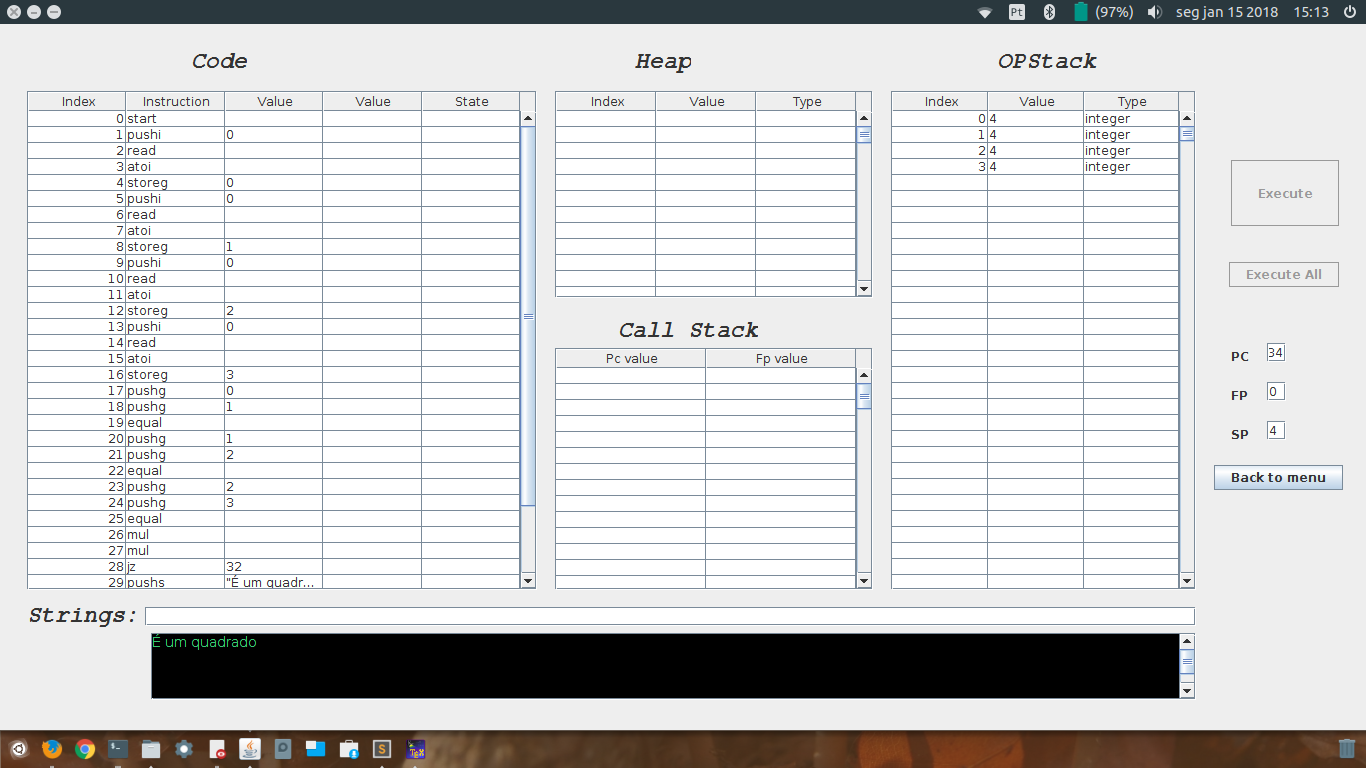
\includegraphics[width=14cm,height= 8cm]{exemplo1-1.png}
	\caption{Verifica se é um quadrado}
	\label{Exemplo 1.1}
\end{figure}

\begin{figure}[h]
	\centering
	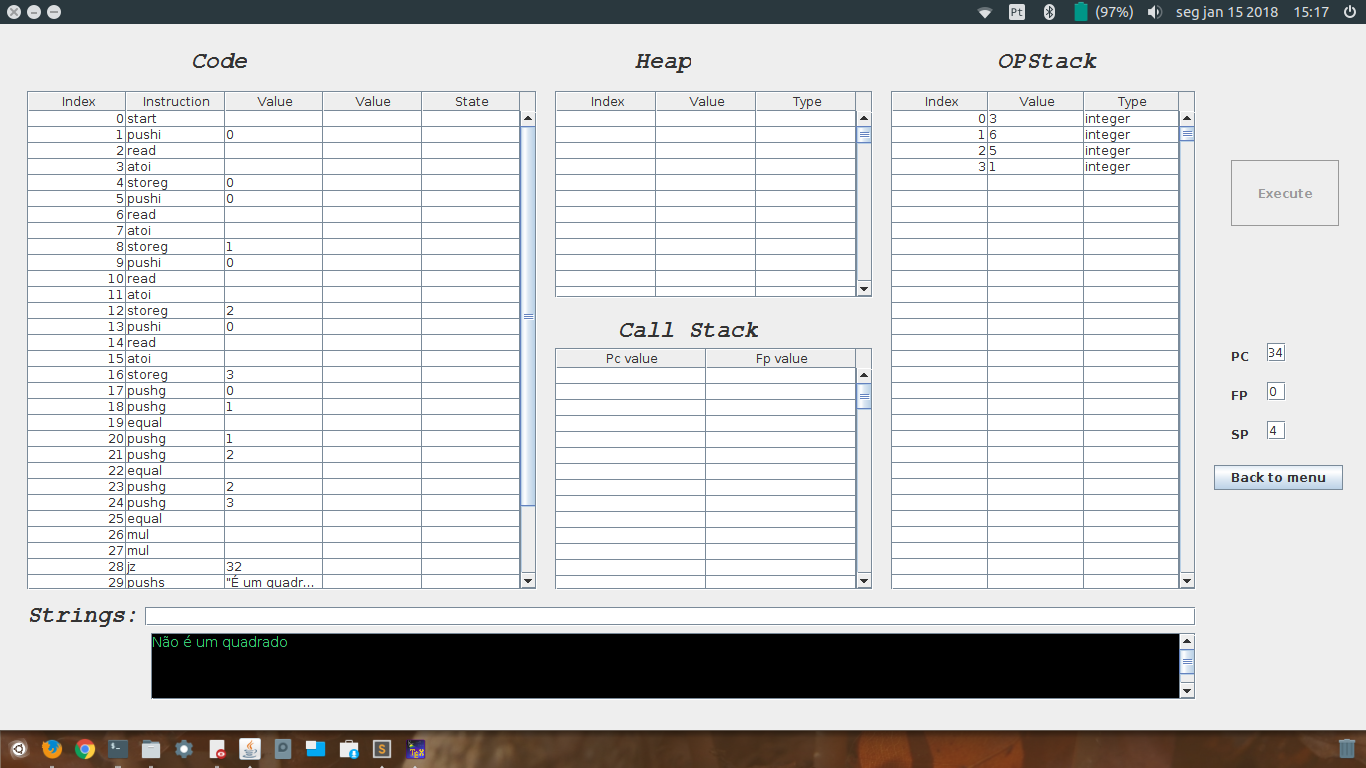
\includegraphics[width=14cm,height= 8cm]{exemplo1-2.png}
	\caption{Verifica que não é um quadrado}
	\label{Exemplo 1.2}
\end{figure}

\begin{figure}[h]
	\centering
	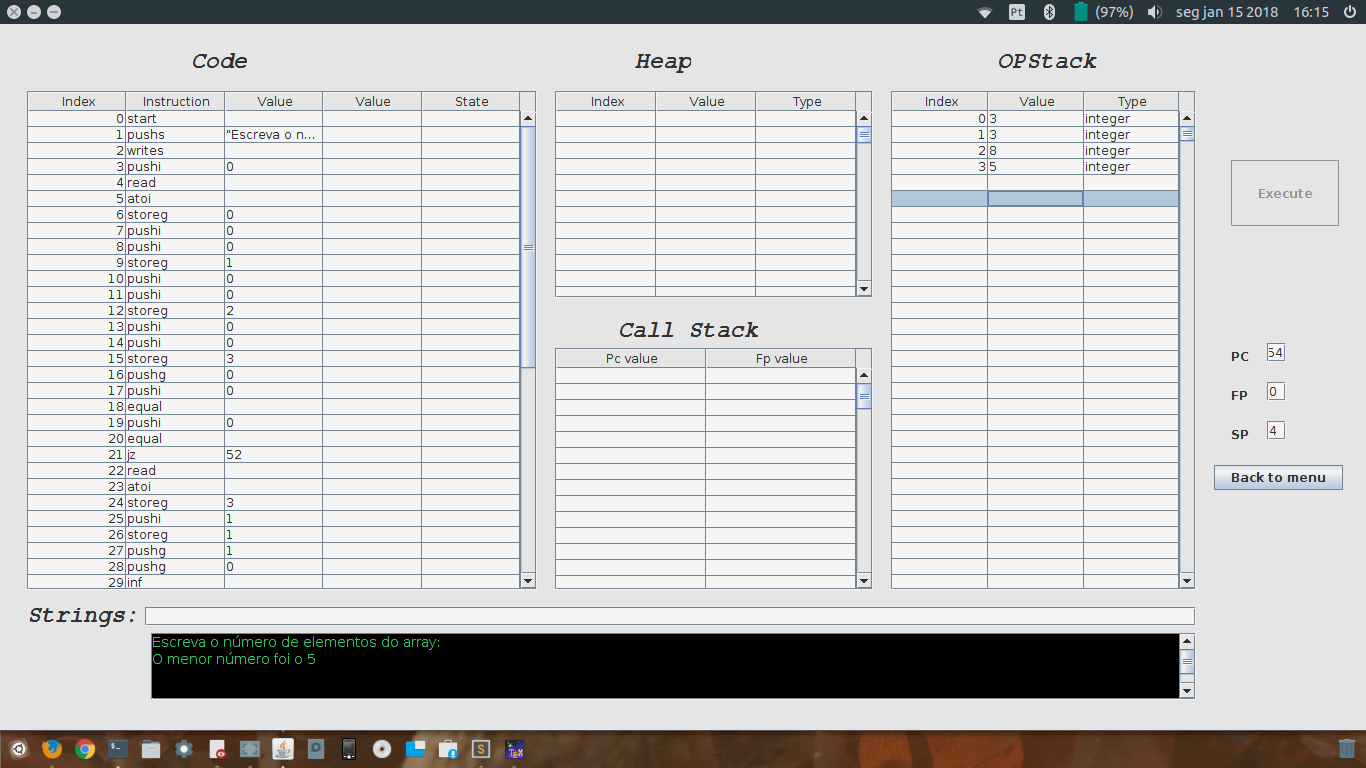
\includegraphics[width=14cm,height= 8cm]{exemplo2-1.png}
	\caption{Diz qual é o menor número}
	\label{Exemplo 2.1}
\end{figure}

\begin{figure}[h]
	\centering
	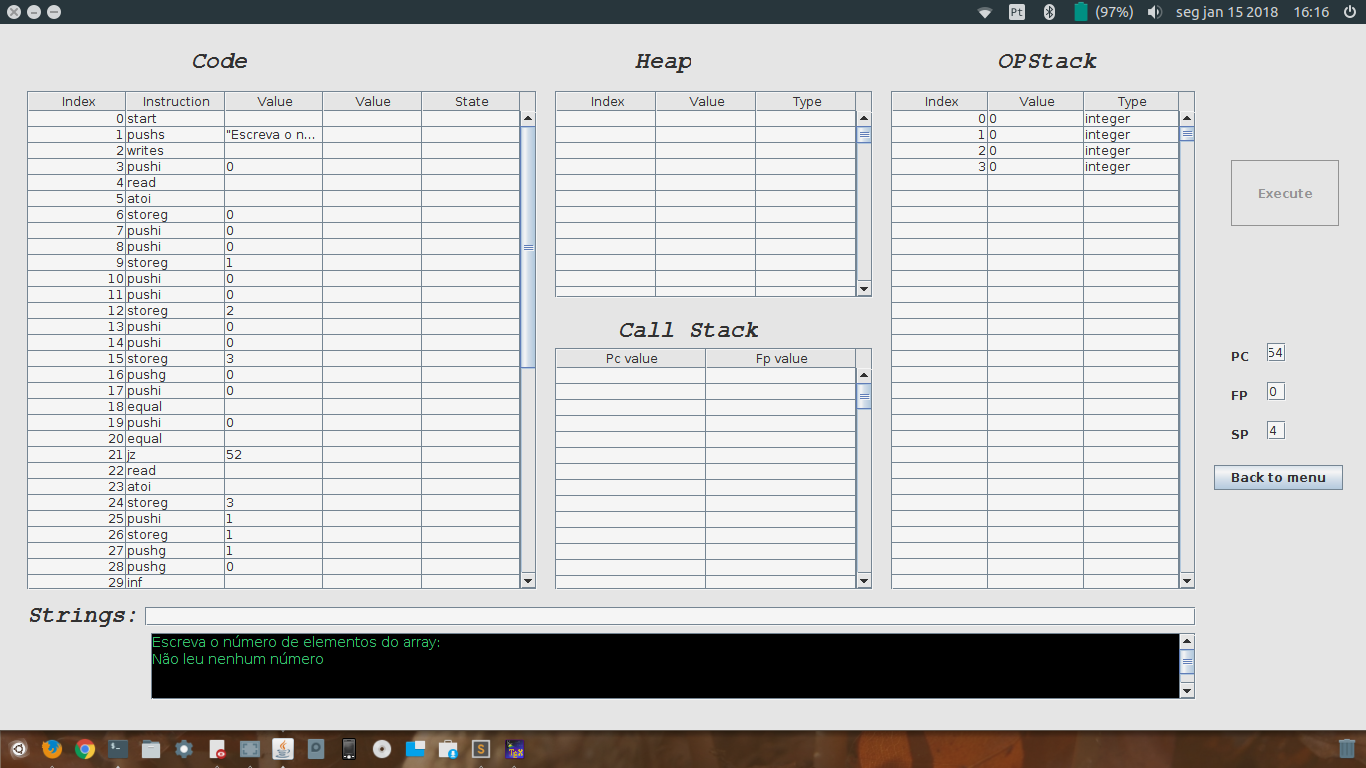
\includegraphics[width=14cm,height= 8cm]{exemplo2-2.png}
	\caption{Verifica que não leu nenhum número}
	\label{Exemplo 2.2}
\end{figure}

\begin{figure}[h]
	\centering
	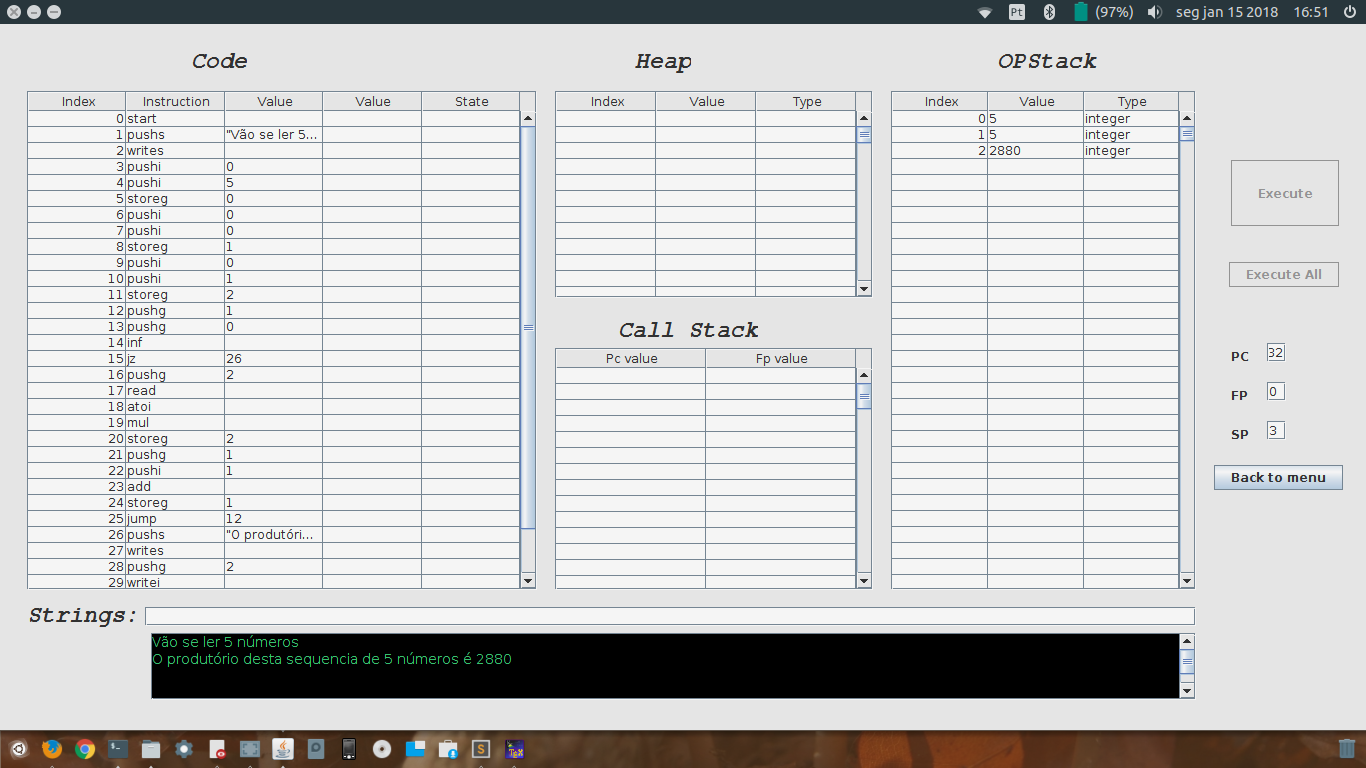
\includegraphics[width=14cm,height= 8cm]{exemplo3-1.png}
	\caption{Apresenta o produtório}
	\label{Exemplo 3.1}
\end{figure}

\begin{figure}[h]
	\centering
	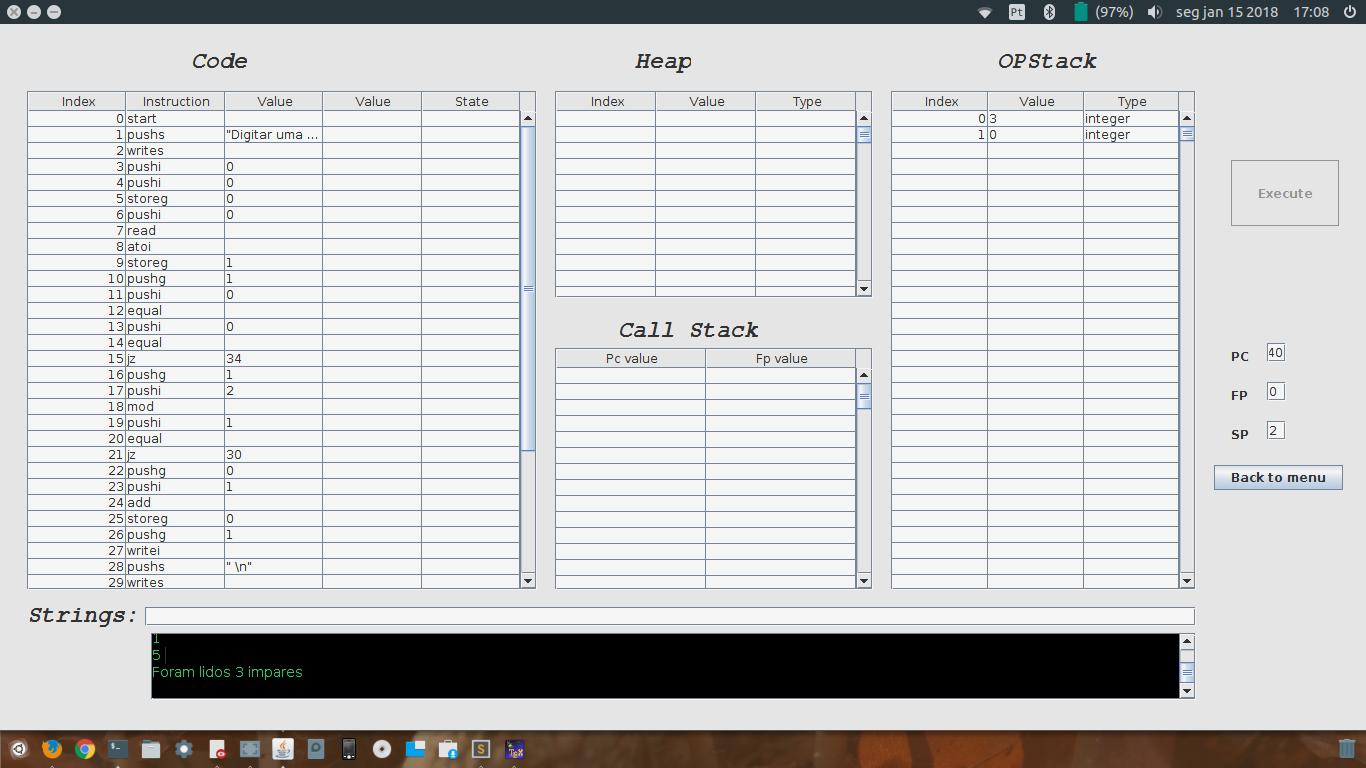
\includegraphics[width=14cm,height= 8cm]{exemplo4-1.png}
	\caption{Mostra quantos impares foram lidos}
	\label{Exemplo 4.1}
\end{figure}

\begin{figure}[h]
	\centering
	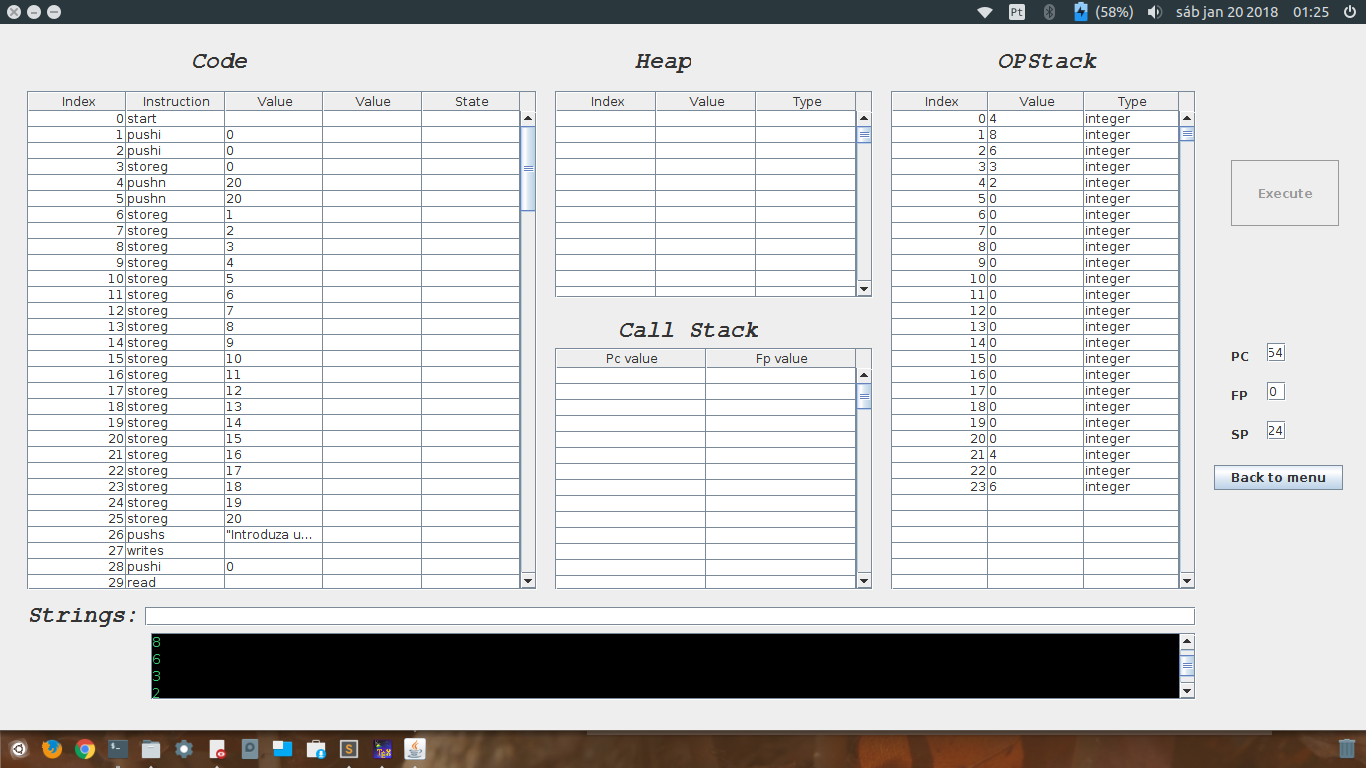
\includegraphics[width=14cm,height= 8cm]{Exemplo5-1.png}
	\caption{Coloca os elemetos do array por ondem ascendente}
	\label{Exemplo 5.1}
\end{figure}

\begin{figure}[h]
	\centering
	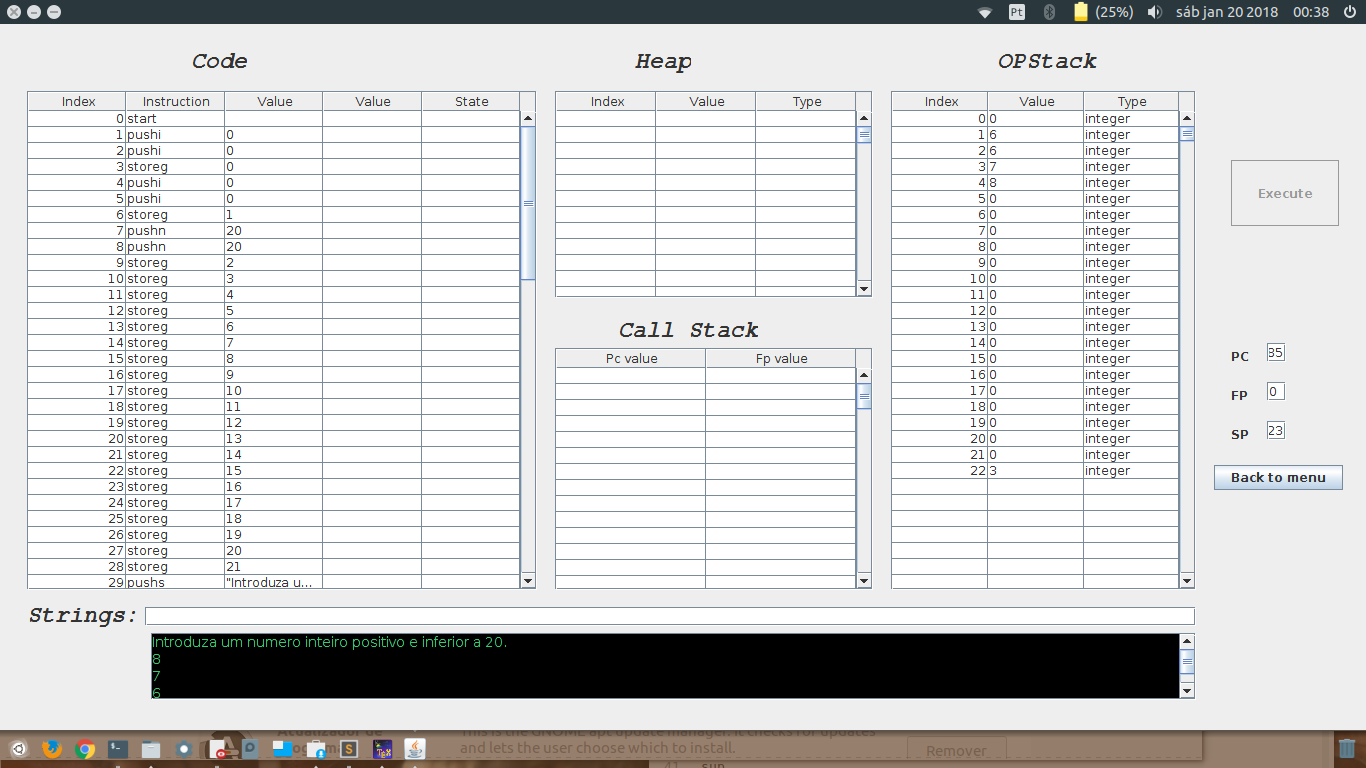
\includegraphics[width=14cm,height= 8cm]{exemplo6-1.png}
	\caption{Mostra os elemetos do array pela ondem inversa}
	\label{Exemplo 6.1}
\end{figure}

\chapter{Código do Programa}
Só o ficheiro galo.l
\begin{code}
%{
#include "y.tab.h"
%}

%%
#.*$                        { return(COM); }
\"[^"]*\"                   { yylval.s = strdup(yytext); return(STR); }
[ ]+e[ ]+                   { return(E); }
[ ]+ou[ ]+                  { return(OU); }
[ ]+sin[ ]+                 { return(SIN); }
[ ]+cos[ ]+                 { return(COS); }
==                          { return(EQ); }
\<=                         { return(LEQ); }
\>=                         { return(GEQ); }
!=                          { return(NEQ); }
[=;{}(),<>!\+\-\*\/%\[\]]   { return(yytext[0]); }
se|SE                       { return(SE); }
senao|SENAO                 { return(SENAO); }
enq|ENQ                     { return(ENQ); }
return                      { return(RETURN); }
[0-9]+\.[0-9]+              { yylval.f = atof(yytext); return(FLOAT); }
int|string|float            { yylval.s = strdup(removeEspacos(yytext)); return(TIPO); }
-?[0-9]+                      { yylval.i = atoi(yytext); return(NUM); }
[a-zA-Z][a-zA-Z0-9]*        { yylval.s = strdup(yytext); return(VAR); }
[ \t\n]                     { ; }
.                           { printf("Caracter invalido %c\n", yytext[0]); }
	%%
	
	int yywrap(){
		return(1);
	}						
							
\end{code}
Ficheiro do Yacc
\begin{code}

%{
#include <stdio.h>
#include <stdlib.h>
#include <string.h>
#define MAX 1024

int yylex();
int yyerror();
int topo = 0, topol = 0, i = 0;
int numse[128] = {0}, apse = 0, numenq[128] = {0}, apenq = 0;
int numelemfun = 0, numfun = 0, dentrofun = 0; 
FILE* out;
char* tipoString = "string";
char* tipoInt = "int";
char* tipoFloat = "float";

typedef struct variavel{
	int   dimensao1;
	int   dimensao2;
	char* tipo;
	char* designacao;
	int   posicaoStack;
} *Variavel;

typedef struct funcao{
	char* designacao;
	char* tipos[128];
	int numtipos;
} *Funcao;

Variavel v[MAX] = {0}, aux = NULL, vl[MAX] = {0};
Funcao funcoes[128] = {0}, funaux = NULL;
int quant = 0, quantl = 0;
char* tiposaux[128] = {0};

int removeVarDesig (char* designacao, Variavel v[], int N){
	if(N==0)return -1;
	int x , y = 0;
	for(x = 0; x<MAX && y<N ; x++){
		if(v[x]!=NULL) y++;
		if(strcmp(v[x]->designacao, designacao)==0){
			v[x] = NULL;
			return N--;
		}
	}
	return -1;
	
}

int insereVar (Variavel var, Variavel v[], int N){
	N = removeVarDesig(var->designacao,v,N);
	if(N>=MAX) return -1;
	
	int x;
	for(x = 0; x<MAX ; x++){
		if(v[x]==NULL) break;	 
	}
	v[x] = var;
	return N++;
}

int removeVar (Variavel var, Variavel v[], int N){
	if(N==0)return -1;
	int x , y = 0;
	for(x = 0; x<MAX && y<N ; x++){
		if(v[x]!=NULL) y++;
		if(v[x]->posicaoStack == var->posicaoStack){
			v[x] = NULL;
			return N--;
		}
	}
	return -1;
}

Variavel criaVar (char* tipo, char* designacao , int posicaoStack, int dimensao1, int dimensao2){
	Variavel var = (Variavel)malloc(sizeof(struct variavel));
	var->dimensao1 = dimensao1;
	var->dimensao2 = dimensao2;
	var->tipo = tipo;
	var->designacao = designacao;
	var->posicaoStack = posicaoStack;
	return var;
}

int isapontador (char* t){
	int i;
	for (i=0; t[i]!='\0'; i++);
	return t[i-1]=='*';
}

char* removeEspacos(char* s){
	int i = 0, j = 0;
	while(s[j]!='\0'){
		while(s[j]==' '){j++;}
		if(s[j]=='\0') break;
		s[i] = s[j];
		i++;j++;
	}
	s[i] = '\0';
	return s;
}

Variavel procuraDesig(char* designacao, Variavel v[], int N){
	int i ,q = 0;
	for(i=0; q<N && i<MAX; i++){
		if(v[i]!=NULL) q++;
		if(strcmp(v[i]->designacao,designacao)==0){
			return v[i];
		}
	}
	return NULL;
	
}

void push(Variavel v){
	if(strcmp(v->tipo,"int")==0){
		if(v->dimensao1==0 && v->dimensao2==0){
			fprintf(out,"pushi 0\n");  
		}else if(v->dimensao1!=0 && v->dimensao2==0){
			fprintf(out,"pushn %d\n",v->dimensao1);
		}else{
			fprintf(out,"pushn %d\n",v->dimensao1*v->dimensao2);
		}
	}else if (strcmp(v->tipo,"string")==0){
		fprintf(out,"pushs \"\"\n");
	}else if (strcmp(v->tipo,"float")==0){
		fprintf(out,"pushf 0.0\n");
	}else {
		printf("ERRO: tipo nao existe");   
	}
	
}

void pushtipo(char* tipo){
	if(strcmp(tipo,"int")==0){
		fprintf(out,"pushi 0\n");  
	}else if (strcmp(tipo,"string")==0){
		fprintf(out,"pushs \"\"\n");
	}else if (strcmp(tipo,"float")==0){
		fprintf(out,"pushf 0.0\n");
	}else {
		printf("ERRO: tipo nao existe");   
	}
	
}

void store(Variavel v){
	fprintf(out,"storeg %d\n",v->posicaoStack);
}

void storel(Variavel v){
	fprintf(out,"storel %d\n",v->posicaoStack);
}

void inserefun(Funcao fun, Funcao funcoes[], int numfun){
	funcoes[numfun] = fun;
}

Funcao criafun(char* designacao, char* tipos[], int numtipos){
	Funcao fun = (Funcao)malloc(sizeof(struct funcao));
	fun->designacao = designacao;
	int i;
	for(i=0;i<numtipos;i++){
		fun->tipos[i] = tipos[i];
	}
	fun->numtipos = numtipos;
	return fun;
}

Funcao atualizafun(Funcao fun, char* tipos[], int numtipos){
	int i;
	for (i=fun->numtipos;i<fun->numtipos+numtipos;i++){
		fun->tipos[i] = tipos[i-fun->numtipos];
	}
	fun->numtipos += numtipos;
	return fun;
}

Funcao procurafun(char* designacao, Funcao funcoes[], int numfun ){
	int i;
	for(i=0;i<numfun;i++){
		if(strcmp(funcoes[i]->designacao,designacao)==0){
			return funcoes[i];
		}
	}
	return NULL;
}

void zerar(Variavel vl[], int quantl){
	Variavel aux = NULL;
	int i = 0;
	while(i<quantl){
		if(vl[i]){
			aux = vl[i];
			vl[i] = NULL;
			free(aux);
			i++;
		}
	}
}
%}

%union{
int i;
float f;
char *s;
Funcao fun;
}


%token SE SENAO ENQ VAR TIPO NUM FLOAT EQ NEQ LEQ GEQ E OU STR COM RETURN COS SIN

%type<i> NUM
%type<f> FLOAT
%type<s> VAR TIPO STR

%type<s> Prog Atrib Se Lexpr Eexpr Ltipo Funcao 
%type<i> Cond
%type<s> Expr Sexpr 


%%
ProgG   : ProgG Se                              { printf("se\n"); }
	| ProgG Enq                             { printf("enquanto\n"); }
	| ProgG Atrib ';'                       { printf("inicializa var\n"); }
	| ProgG VAR '=' Expr ';'                { printf("atualiza var\n"); store(procuraDesig($2,v,quant)); }
	| ProgG IgualL ';'                      { printf("atualiza vetor\n"); }
	| ProgG CriaFun                         { printf("declarar funcao\n");}
	| ProgG Funcao ';'                      { printf("chamar funcao\n"); }
	| ProgG ';'                             { printf("; desnecessario\n"); } 
	| ProgG COM                             { printf("comentario\n"); } 
	|                                       { printf("inicio\n"); } 
	;

ProgF   : ProgF Se                              { printf("se\n"); }
	| ProgF Enq                             { printf("enquanto\n"); }
	| ProgF Atrib ';'                       { printf("inicializa var\n"); }
	| ProgF VAR '=' Expr ';'                { printf("atualiza var\n"); store(procuraDesig($2,vl,quantl)); }
	| ProgF IgualL ';'                      { printf("atualiza vetor\n"); }
	| ProgF Funcao ';'                      { printf("chamar funcao\n"); }
	| ProgF ';'                             { printf("; desnecessario\n"); } 
	| ProgF COM                             { printf("comentario\n"); } 
	| ProgF RETURN Expr ';'                 { printf("return\n"); fprintf(out,"storel 
						%d\nreturn\n",-(numelemfun+1)); } 
	|                                       { printf("inicio\n"); } 
	;

Prog    : Prog Se                               { printf("se\n"); }
	| Prog Enq                              { printf("enquanto\n"); }
	| Prog Atrib ';'                        { printf("inicializa var\n"); }
	| Prog VAR '=' Expr ';'                 { printf("atualiza var\n"); store(procuraDesig($2,v,quant)); }
	| Prog IgualL ';'                       { printf("atualiza vetor\n"); }
	| Prog Funcao ';'                       { printf("chamar funcao\n"); }
	| Prog ';'                              { printf("; desnecessario\n"); } 
	| Prog COM                              { printf("comentario\n"); } 
	|                                       { printf("inicio\n"); } 
	;

Funcao  : VAR Lexpr                             { if(strcmp($1,"leri")==0){
		fprintf(out,"read\natoi\n");
		$$ = tipoInt;
	}else if(strcmp($1,"lerf")==0){
		fprintf(out,"read\natof\n");
		$$ = tipoFloat;
	}else if(strcmp($1,"lers")==0){
		fprintf(out,"read\n");
		$$ = tipoString;
	}else if(strcmp($1,"escreveri")==0){
		fprintf(out,"writei\n");
		$$ = tipoInt;
	}else if(strcmp($1,"escrevers")==0){
		fprintf(out,"writes\n");
		$$ = tipoString;
	}else if(strcmp($1,"escreverf")==0){
		fprintf(out,"writef\n");
		$$ = tipoFloat;
	}else if(strcmp($1,"atoi")==0){
		fprintf(out,"atoi\n");
		$$ = tipoInt;
	}else if(strcmp($1,"atof")==0){
		fprintf(out,"atof\n");
		$$ = tipoFloat;
	}else if(strcmp($1,"ftoi")==0){
		fprintf(out,"ftoi\n");
		$$ = tipoInt;
	}else if(strcmp($1,"itof")==0){
		fprintf(out,"itof\n");
		$$ = tipoFloat;
	}else if(strcmp($1,"stri")==0){
		fprintf(out,"stri\n");
		$$ = tipoString;
	}else if(strcmp($1,"strf")==0){
		fprintf(out,"strf\n");
		$$ = tipoString;
	}else{
		funaux = procurafun($1,funcoes,numfun);
		if(!funaux){
			printf("ERRO: funcao nao encontrada\n");
		}else{
			$$ = funaux->tipos[0];
			pushtipo(funaux->tipos[0]);
			for(i=0;i<numelemfun;i++){
				fprintf(out,"pushl %d\n",topo+numelemfun-i-1);
			}
			fprintf(out,"pusha %s\ncall\nnop\npop %d\n",$1,numelemfun);
			for(i=0;i<numelemfun;i++){
				fprintf(out,"swap\npop 1\n");
			}
		}
	}
}
;

CriaFun : TIPO VAR '('                   { fprintf(out,"jump fimfun%d\n%s:\nnop\n",numfun,$2); dentrofun = 1; 
	inserefun(criafun($2,&$1,1),funcoes,numfun); 
}
| Ltipo '{' ProgF '}'                   { fprintf(out,"fimfun%d:\n",numfun); numfun++; dentrofun = 0; zerar(vl,quantl); quantl = 0; }
	;
	
	Atrib   : TIPO VAR                              { if(dentrofun){
			aux = criaVar($1,$2,topol++,0,0);
			insereVar(aux, vl, quantl++);
			push(aux); push(aux); storel(aux);
		}
		else{
			aux = criaVar($1,$2,topo++,0,0);
			insereVar(aux, v, quant++); 
			push(aux); push(aux); store(aux);
		} 
	} 
	| TIPO VAR '[' NUM ']'                 { if(dentrofun){
			aux = criaVar($1,$2,topol,$4,0); topol += $4;
			insereVar(aux, vl, quantl++);
			push(aux); push(aux); 
			for(i=0;i< $4;i++){
				fprintf(out,"storel %d\n",(i+aux->posicaoStack));
			}
		}
		else{
			aux = criaVar($1,$2,topo,$4,0); topo += $4;
			insereVar(aux, v, quant++); 
			push(aux); push(aux);
			for(i=0;i< $4;i++){
				fprintf(out,"storeg %d\n",(i+aux->posicaoStack));
			}
		}
	} 
	| TIPO VAR '[' NUM ',' NUM ']'         { if(dentrofun){
			aux = criaVar($1,$2,topol,$4,$6); topol += $4*$6;
			insereVar(aux, vl, quantl++);
			push(aux); push(aux);
			for(i=0;i< $4*$6;i++){
				fprintf(out,"storel %d\n",(i+aux->posicaoStack));
			}
		}
		else{
			aux = criaVar($1,$2,topo,$4,$6); topo += $4*$6;
			insereVar(aux, v, quant++); 
			push(aux); push(aux);
			for(i=0;i< $4*$6;i++){
				fprintf(out,"storeg %d\n",(i+aux->posicaoStack));
			}
		}
	}
	| Igual                                 { ; }       
	;
	
	Igual   : TIPO VAR '='                          { if(dentrofun){
			aux = criaVar($1,$2,topol++,0,0);
			insereVar(aux, vl, quantl++);
			push(aux);
		}
		else{
			aux = criaVar($1,$2,topo++,0,0); 
			insereVar(aux, v, quant++);
			push(aux);
		}
	}
	| Igual Expr                            { if(dentrofun){
			storel(aux);
		}
		else{
			store(aux);
		} 
	}
	;
	
	IgualL  : VAR '[' Expr ']'                      { if(dentrofun){        
			fprintf(out,"pushi %d\nadd\npushgp\nswap\n",procuraDesig($1,vl,quantl)->posicaoStack);
		}else{
			fprintf(out,"pushi %d\nadd\npushgp\nswap\n",procuraDesig($1,v,quant)->posicaoStack);
		}
	}
	| IgualL '=' Expr                       { fprintf(out,"storen\n"); }
	
	/*lista de expressoes*/
	Lexpr   : '(' ')'                               { numelemfun = 0; }
	| '(' Eexpr ')'                         { ; }
	;
	
	Eexpr   : Expr                                  { numelemfun = 1; }
	| Eexpr ',' Expr                        { numelemfun++; }
	;
	
	/*lista de tipos*/
	Ltipo   : ')'                                   { numelemfun = 0; }
	| Etipo ')'                             { ; }
	;
	
	Etipo   : TIPO VAR                              { numelemfun = 1; aux = criaVar($1,$2,-(numelemfun),0,0);
		insereVar(aux, vl, quantl++); atualizafun(funcoes[numfun],&$1,1);  
	}
	| Etipo ',' TIPO VAR                    { numelemfun++; aux = criaVar($3,$4,-(numelemfun),0,0);
		insereVar(aux, vl, quantl++); atualizafun(funcoes[numfun],&$3,1); 
	}
	;
	
	Se      : SE Cond                               { fprintf(out, "jz fimse%d\n",numse[apse]); apse++; numse[apse] = numse[apse-1]+1; }
		| Se '{' Prog '}' SENAO                 { apse--; fprintf(out, "jump fimse%d\nfimse%d:\n",numse[apse+1],numse[apse]);
			numse[apse] = numse[apse+1]; apse++; numse[apse] = numse[apse-1]+1; 
		}
		| Se '{' Prog '}'                       { apse--; fprintf(out, "fimse%d:\n",numse[apse]); numse[apse] = numse[apse+1]; }
			;
			
			Enq     : ENQ                                   { fprintf(out,"enq%d:\n",numenq[apenq]); }
				| Enq Cond                              { fprintf(out,"jz fimenq%d\n",numenq[apenq]); apenq++; numenq[apenq] = numenq[apenq-1]+1; }
					| Enq '{' Prog '}'                      { apenq--; fprintf(out,"jump enq%d\nfimenq%d:\n",numenq[apenq],numenq[apenq]); 
						numenq[apenq]= numenq[apenq+1]; 
					}
					;
					
					Cond    : NUM                                   { fprintf(out,"pushi %d\n",$1!=0); }
						| '(' Expr EQ Expr ')'                  { fprintf(out,"equal\n"); }
						| '(' Expr NEQ Expr ')'                 { fprintf(out,"equal\npushi 0\nequal\n"); }
						| '(' Expr '<' Expr ')'                 { if(strcmp($2,"int")==0 && strcmp($4,"int")==0){
								fprintf(out,"inf\n");
							}else if(strcmp($2,"float")==0 && strcmp($4,"float")==0){
								fprintf(out,"finf\nftoi\n");
							}else{
								printf("ERRO: tipos sem sentido na condicao.\n");
							}
						}
						| '(' Expr '>' Expr ')'                 { if(strcmp($2,"int")==0 && strcmp($4,"int")==0){
								fprintf(out,"sup\n");
							}else if(strcmp($2,"float")==0 && strcmp($4,"float")==0){
								fprintf(out,"fsup\nftoi\n");
							}else{
								printf("ERRO: tipos sem sentido na condicao.\n");
							}
						}
						| '(' Expr LEQ Expr ')'                 { if(strcmp($2,"int")==0 && strcmp($4,"int")==0){
								fprintf(out,"infeq\n");
							}else if(strcmp($2,"float")==0 && strcmp($4,"float")==0){
								fprintf(out,"finfeq\nftoi\n");
							}else{
								printf("ERRO: tipos sem sentido na condicao.\n");
							}
						}
						| '(' Expr GEQ Expr ')'                 { if(strcmp($2,"int")==0 && strcmp($4,"int")==0){
								fprintf(out,"supeq\n");
							}else if(strcmp($2,"float")==0 && strcmp($4,"float")==0){
								fprintf(out,"fsupeq\nftoi\n");
							}else{
								printf("ERRO: tipos sem sentido na condicao.\n");
							}
						}
						| '(' Cond E Cond ')'                   { fprintf(out,"mul\n"); }
						| '(' Cond OU Cond ')'                  { fprintf(out,"add\n"); }
						| '!' Cond                              { fprintf(out,"pushi 0\nequal\n"); }
						;
						
						Sexpr   : VAR                                   { if(dentrofun){
								aux = procuraDesig($1,vl,quantl);
								fprintf(out,"pushl %d\n",aux->posicaoStack); 
							}else{
								aux = procuraDesig($1,v,quant);
								fprintf(out,"pushg %d\n",aux->posicaoStack); 
							}
							$$ = aux->tipo;
						}
						| NUM                                   { fprintf(out,"pushi %d\n", $1); $$ = tipoInt; }
							| FLOAT                                 { fprintf(out,"pushf %f\n", $1); $$ = tipoFloat; }
								| VAR '[' Expr ']'                      { if(dentrofun){
										aux = procuraDesig($1,vl,quantl);
										fprintf(out,"pushi %d\nadd\npushgp\nswap\nloadn\n", procuraDesig($1,vl,quantl)->posicaoStack);
									}else{
										aux = procuraDesig($1,v,quant);
										fprintf(out,"pushi %d\nadd\npushgp\nswap\nloadn\n", procuraDesig($1,v,quant)->posicaoStack);
									}
									$$ = aux->tipo;
								}
								| Funcao                                { $$ = $1; } 
								| STR                                   { fprintf(out,"pushs %s\n", $1); $$ = tipoString; }
									;
									
									Expr	: '(' Expr '+' Expr ')'    			    { if(strcmp($2,"int")==0 && strcmp($4,"int")==0){
											fprintf(out,"add\n");
											$$ = $2;
										}else if(strcmp($2,"float")==0 && strcmp($4,"float")==0){
											fprintf(out,"fadd\n");
											$$ = $2;
										}else if(strcmp($2,"string")==0 && strcmp($4,"string")==0){
											fprintf(out,"concat\n");
											$$ = $2;
										}else{
											printf("ERRO: Na operacao '+' tipos sem sentido\n");
										}
									}
									| '(' Expr '-' Expr ')'  	            { if(strcmp($2,"int")==0 && strcmp($4,"int")==0){
											fprintf(out,"sub\n");
											$$ = $2;
										}else if(strcmp($2,"float")==0 && strcmp($4,"float")==0){
											fprintf(out,"fsub\n");
											$$ = $2;
										}else{
											printf("ERRO: Na operacao '-' tipos sem sentido\n");
										} 
									}
									| '(' Expr '*' Expr ')'    	            { if(strcmp($2,"int")==0 && strcmp($4,"int")==0){
											fprintf(out,"mul\n");
											$$ = $2;
										}else if(strcmp($2,"float")==0 && strcmp($4,"float")==0){
											fprintf(out,"fmul\n");
											$$ = $2;
										}else{
											printf("ERRO: Na operacao '*' tipos sem sentido\n");
										} 
									}
									| '(' Expr '/' Expr ')'    	            { if(strcmp($2,"int")==0 && strcmp($4,"int")==0){
											fprintf(out,"div\n");
											$$ = $2;
										}else if(strcmp($2,"float")==0 && strcmp($4,"float")==0){
											fprintf(out,"fdiv\n");
											$$ = $2;
										}else{
											printf("ERRO: Na operacao '/' tipos sem sentido\n");
										} 
									}
									| '(' Expr '%' Expr ')'    	            { if(strcmp($2,"int")==0 && strcmp($4,"int")==0){
									fprintf(out,"mod\n");
									$$ = $2;
								}else{
									printf("ERRO: Na operacao '%%' tipos sem sentido\n");
								} 
							}
							| COS Expr                              { if(strcmp($2,"float")==0){
									fprintf(out,"fcos\n");
									$$ = $2;
								}else{
									printf("ERRO: Na operacao 'cos' tipos sem sentido\n");
								} 
							}
							| SIN Expr                              { if(strcmp($2,"float")==0){
									fprintf(out,"fsin\n");
									$$ = $2;
								}else{
									printf("ERRO: Na operacao 'sin' tipos sem sentido\n");
								} 
							}
							| '(' Expr ')'                          { $$ = $2; }
							| Sexpr                                 { $$ = $1; }
							;
							%%
							
							#include "galo.c"
							
							int yyerror(char *s){
								fprintf(stderr, "ERRO SINTATICO: %s \n", s);
							}
							
							int main(){
								out = fopen("a.vm", "w");
								if (out == NULL){
									printf("Error opening file!\n");
									exit(1);
								}
								//char codigo[1023*1024];
								fprintf(out, "start\n"); 
								yyparse();
								fprintf(out, "stop\n");
								
								fclose(out);
								return(0);
							}
	
\end{code}



\end{document}